\documentclass[tikz,border=8pt]{standalone}
\usepackage{lmodern}
\usetikzlibrary{arrows.meta,positioning}
\begin{document}
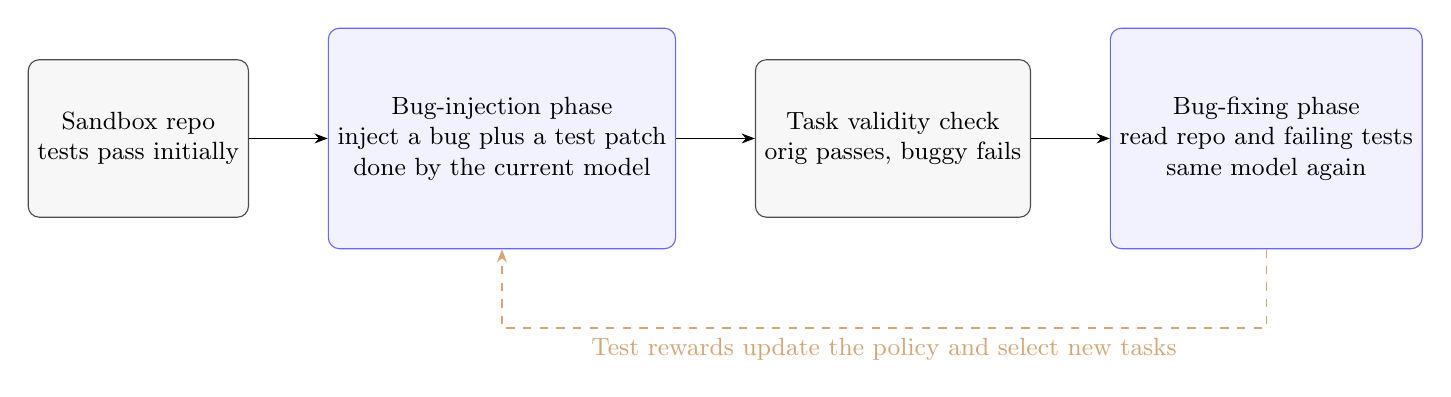
\begin{tikzpicture}[node distance=10mm,>=Stealth,every node/.style={align=center,font=\small},box/.style={rounded corners,draw=black!70,fill=black!3,minimum height=20mm},role/.style={box,draw=blue!60,fill=blue!5,minimum height=28mm}]
\node[box] (repo) {Sandbox repo\\tests pass initially};
\node[role,right=of repo] (inject) {Bug-injection phase\\inject a bug plus a test patch\\done by the current model};
\node[box,right=of inject] (check) {Task validity check\\orig passes, buggy fails};
\node[role,right=of check] (repair) {Bug-fixing phase\\read repo and failing tests\\same model again};
\draw[->] (repo)--(inject); \draw[->] (inject)--(check); \draw[->] (check)--(repair);
\draw[->,dashed,brown!70] (repair.south) -- ++(0,-10mm) -| node[below,pos=.25]{Test rewards update the policy and select new tasks} (inject.south);
\end{tikzpicture}
\end{document}
